\documentclass[a4paper]{article}
\usepackage[utf8]{inputenc}
\usepackage{textcomp}
\usepackage{geometry}
\geometry{ left=2cm, right=2cm, top=2cm, bottom=2cm, bindingoffset=5mm}
\usepackage{graphicx}
\usepackage{xcolor}
\usepackage{hyperref}
\date{}
\author{}
\usepackage{fancyhdr}
\pagestyle{fancy}
\fancyhf{}
\fancyhead[R]{2973140 - Felix Bühler  \\ 2893121 - Jan Leusmann \\  3141241 - Jamie Ullerich}
\fancyhead[L]{Reinforcement Learning \\ SS 2020}
\renewcommand{\headrulewidth}{0.5pt}
\usepackage{tikz}
\usetikzlibrary{calc}
\usepackage{amsmath}
\usepackage{cleveref}
\usepackage{subcaption}
\usepackage{array}
\usepackage{bbold}

\title{\textbf{Exercise 1}}

\begin{document}
\maketitle 
\thispagestyle{fancy}

\section*{Task 1 - Multi-armed Bandits}

\begin{enumerate}
	\item[a)] The probability that the greedy action is selected is $1- \epsilon = 1 - 0.5 = 0.5$ 
	% ist es wichtig das es k=2 actions gibt?
	\item[b)] A random action definitely occurred at time step 2 and 5, and could possibly have occurred at time step 1 and 3.\\
	Calculate $Q_t(a) = \dfrac{\sum_{i=1}^{t-1}R_i \cdot \mathbb{1}_{A_i = a}}{\sum_{i=1}^{t-1} \mathbb{1}_{A_i = a}}$ for each action and time step $\rightarrow$ if the action with the largest value was taken, a greedy action occurred, otherwise it would be random. \\
	\begin{tabular}{>{$}l<{$} >{$}l<{$} >{$}l<{$} c c c}
		& & & $\underset{a}{\mathrm{arg \ max}} Q_t(a)$ & $A_t$ & $R_t$\\
		Q_1(1) = 0 &  Q_1(2) = 0 & Q_1(3) = 0 & 1, 2, 3 & 1 & 1\\
		Q_2(1) = 1 &  Q_2(2) = 0 & Q_2(3) = 0 & 1 &2 & 1\\
		Q_3(1) = 1 &  Q_3(2) = 1 & Q_3(3) = 0 & 1, 2& 2 & 2\\
		Q_4(1) = 1 &  Q_4(2) = 3 & Q_4(3) = 0 & 2& 2 & 2\\
		Q_5(1) = 1 &  Q_5(2) = 5 & Q_5(3) = 0 & 2& 3 & 0\\
	\end{tabular}
\end{enumerate}

\section*{Task 2 - Action Selection Strategies}

\subsection*{c)}

epsilon greedy search performs better, as it also includes exploration and not only exploitation.

\begin{figure}[!ht]
	\centering
	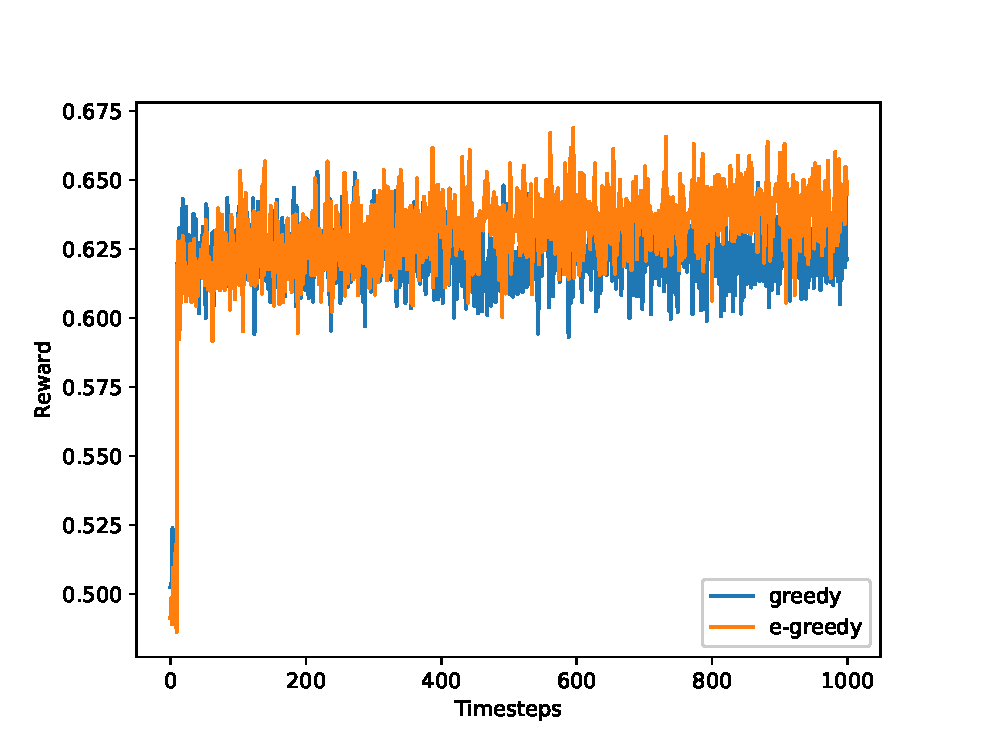
\includegraphics[width=0.7\linewidth]{bandit_strategies}
	\caption{Output bandit\_strategies.eps}
	\label{fig:banditstrategies}
\end{figure}


\subsection*{d)} 
decay epsilon over time.

\end{document}
